%To evaluate the behavior and accuracy of ConPaaS when hosting web applications, we prepared a realistic and complex enough scenario to assess any PaaS. In particular, we deployed the Wikipedia web application called MediaWiki~\cite{mediawiki}, and used a web hosting benchmark called WikiBench~\cite{wikibench}. 

To evaluate the resource provisioning algorithms implemented in ConPaaS,
we prepared a realistic testing scenario: we used a copy of Wikipedia as
the web application, and replayed a fraction of the access traces from
Wikipedia's official web site.  
%In this section, we describe our scenario in detail.

Wikipedia uses MediaWiki~\cite{mediawiki}, a PHP-based wiki software 
package.
%The architecture of the Wikipedia website uses a http-proxy, a http-web server, a database and one or more PhP servers. 
To deploy the Wikipedia services on ConPaaS, we composed two different services: the PHP web hosting and MySQL service. In the MySQL service, we installed a complete copy the database containing English Wikipedia articles from 2008, which has a size of approximately 30GB.
In the PHP service, the configuration was composed of one load balancer,
one static web server and one or more PHP servers. ConPaaS uses nginx
as static web server and also as load balancer. The PHP requests are 
handled through PHP FastCGI Process Manager, known as PHP-FPM.
%In the PhP service, an initial configuration was composed of one Nginx http-proxy, one Apache server, and one or more PhP (FastCGI Process Manager) servers. Each PhP server hosts the MediaWiki application which is the main component of this system. 


%\subsection*{Characteristics of its workload}

%In order to benchmark ConPaaS when hosting the Wikipedia services, we used the WikiBench research tool which generates realistic benchmarks with adaptable traffic properties. WikiBench has a number of advantages compared to the existing benchmark tools for web applications. First of all, Wikibench traces add a high degree of realism, since it is entirely based on the Wikipedia software and data. Indeed, the benchmark workloads are generated based on real access traces from the WikiMedia Foundation. These traces contain detailed  traffic logs of requests made to Wikipedia by its users. As an example, in Figure~\ref{workload}, we show the workload of one trace, as the number of PhP requests per minute during approximately one day.  In this paper, we focus on the behavior of PhP requests which makes particularly difficult to predict their execution times using auto-scaling sytems. 

To evaluate our system we used Wikibench~\cite{wikibench}, a tool for benchmarking Wikipedia 
servers developed by our group. Wikibench replays Wikipedia access
traces or smaller samples of the traces, providing various sampling
mechanisms. We used anonymized Wikipedia access traces, which are 
published by the WikiMedia foundation, and for our experiments we
replayed a sample of 10\% from the traces. The traces contain two 
types of requests: requests for static pages or files, and dynamic
PHP requests. The first performance bottlenecks appear at the logic
tier of the application (the execution of dynamic PHP requests), the static 
requests being executed one order of magnitude faster than the dynamic 
ones. Thus in this article we will focus mostly on the automatic
scaling of the PHP tier.

%Since the original Wikipedia traces can reach peaks of 50000 or 60000 reqs./secs, WikiBench uses the original 10\% sample of these traces which can generate a workload up to about 5000 reqs./secs.

%Even though we use the original 10\% sample of these traces, they are very heterogeneous in terms of workload-mix. To illustrate this heterogeneity, in Figure~\ref{phpRespTimeDispersion}, we present the distribution of the response time values for the PhP requests during the execution of the trace shown in Figure~\ref{workload}. A first observation shows an irregular dispersion of the response time values in two levels: (i) a long-term level on which the values vary along the trace execution without following any clear pattern; and (ii) a short-term level on which the response times widely diverge under short period of time such as one minute. There are two reasons for this dispersion: (i) PhP pages often require database queries; (ii) PhP pages need third-party static files. These issues limits the utilization of provisioning techniques which scale applications only based on current response values. Note that, to obtain response values totally independent of any scaling decisions, we utelementsilized static provisioning to execute this trace. 

As an example, in Figure~\ref{workload}, we show the PHP workload 
sampled from one trace, as the number of PHP requests per minute 
during approximately one day. One aspect that we noticed about the 
workload is that the requests are heterogeneous in complexity.
To illustrate this heterogeneity, in Figure~\ref{phpRespTimeDispersion}
we present the distribution of the response time values for the PHP 
requests during the execution of the trace shown in Figure~\ref{workload}.
For this experiment we used a fixed number of 5 PHP servers,
which are sufficient for handling the workload from the access 
trace even at its peaks; this is why in this case the response 
time is not influenced by the intensity of the workload.  
However, the results show a relatively wide 
dispersion of the response time: the response time values are 
commonly spread between approximately 100 and 300 milliseconds, 
so there is a factor of 3 between the slowest and the fastest requests. 
The main reason for this dispersion is that the Wikipedia articles 
vary in complexity, requiring different amounts of information that
needs to be retrieved from the database and assembled in a page. 

The heterogeneity of the requests makes Wikipedia different from 
some web benchmarking applications, which have a workload mix that
is more homogeneous and predictable; thus we believe that it is a good
choice for achieving a realistic test scenario. We also conclude from
this experiment that, since the response time of the application varies and 
cannot be properly predicted even when the request rate is known, 
a provisioning algorithm aiming to keep the application's response time 
under a certain limit should take into account several monitoring 
parameters (not just the request rate or just the response time).

%Similarly, as depicted by Figure~\ref{workload} and Figure~\ref{phpRespTimeDispersion}, there is not any correlation between the PhP request volumes and their response times. More precisely in Figure~\ref{phpRespTimeDispersion}, the highest response time values obtained in the interval of time 600min. match up with a drop in the request rate during the same interval in Figure~\ref{workload}. Therefore, any provisioning technique that makes decisions based on the request rate can incur errors by under- or over-provisioning an application, which can reduces the efficiency of the scaling actions. 


%I got the expected behavior different response time values independently of the req rate at each time. }

%\fixme{ OTHER POSSIBILITY: More precisely in Figure~\ref{reqRate}, the highest response time values obtained during the trace execution, %match up with low levels of requests rate. Therefore, ...  }

% Similarly, the intensity of the resulting traffic could also be modified ranging from very low up to the 
% original traffic intensity of the trace. 

%Initial benchmark results show a typical day of Wikipedia traffic and the relation between the request rate %and the server response times. 


\begin{figure}
\begin{center}
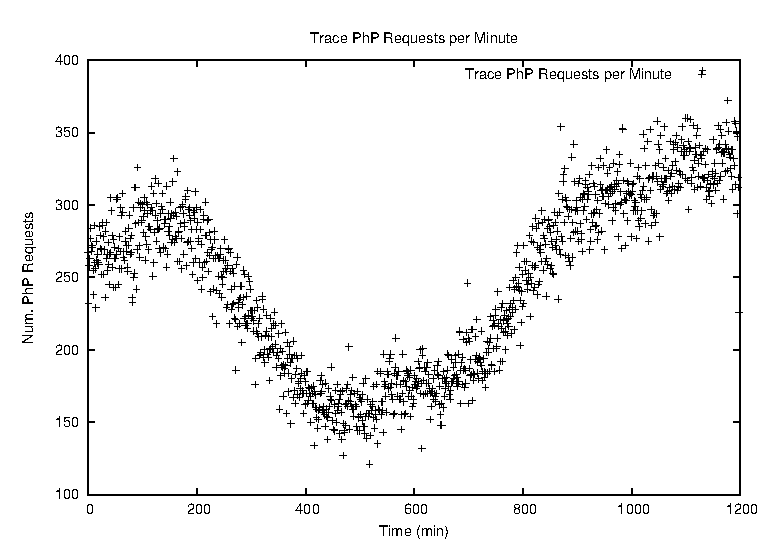
\includegraphics[width=0.49\textwidth, height=6cm]{./images/traceWorkload}
\end{center}
\caption{Wikipedia trace workload.}
\label{workload}
\end{figure}

% Corina - I think this paragraph would be better suitable for future work:
%In addition, other properties may be also considered important when using the Wikipedia traces such as the interarrival time between requests, the distribution of page popularity, the mix of static/dynamic requests, the ratio of read/write operations and requests for non-existing pages and files.

%\begin{itemize}
%\item The intervarrival time between requests follows a Poisson distribution.

%\item The distribution of page popularity varies from very popular pages to those being accessed very infrequently.

%\item The mix of static/dynamic requests presents a strong variation. 

\begin{figure}
\begin{center}
\includegraphics[width=0.49\textwidth, height=6cm]{./images/phpRespTimeDispersion}
\end{center}
\caption{Complexity of PhP requests.}
\label{phpRespTimeDispersion}
\end{figure}

%\item The ratio of read/write operations vary having more reads than editions or creations of wiki pages.

%\begin{figure}
%\begin{center}
%\includegraphics[width=0.49\textwidth, height=6cm]{./images/staticProv_reqRate}
%\end{center}
%\caption{Response time vs request rate.}
%\label{reqRate}
%\end{figure}

%\item A considerable amount of requests for non-existing pages and files add realism to the traffic.

%\end{itemize}


%By using real world server side software and data, we think the WikiBench benchmarking suite is a very  realistic and extensible research tool.

% these traces create workloads for WikiBench instead of creating purely synthetic workloads like other benchmarking tools have done.

%The workload-mix and the variable amount of data and visitors make of Wikipedia a valid example of elastic web application. In this paper, we focus in the scalability of the PhP web hosting service, and thereby as the number of PhP servers hosting MediaWiki scale out or back based on the demanding workload.

